\mbox{$\displaystyle +\,\frac{1}{4}$\,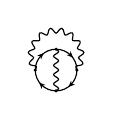
\begin{tikzpicture}[x=0.340cm, y=0.340cm, line width=0.420pt, baseline={([yshift=-0.6ex]0,0)}]
  \draw (-0.778,0.000) arc[start angle=180.000, end angle=90.000, radius=0.778];
  \fill (-0.466,0.634) -- (-0.707,0.538) -- (-0.580,0.520) -- (-0.562,0.393) -- cycle;
  \draw (0.000,0.778) arc[start angle=90.000, end angle=0.000, radius=0.778];
  \fill (0.634,0.466) -- (0.538,0.707) -- (0.520,0.580) -- (0.393,0.562) -- cycle;
  \draw (0.000,-0.778) arc[start angle=270.000, end angle=180.000, radius=0.778];
  \fill (-0.634,-0.466) -- (-0.538,-0.707) -- (-0.520,-0.580) -- (-0.393,-0.562) -- cycle;
  \draw (0.778,0.000) arc[start angle=0.000, end angle=-90.000, radius=0.778];
  \fill (0.466,-0.634) -- (0.707,-0.538) -- (0.580,-0.520) -- (0.562,-0.393) -- cycle;
  \draw plot[smooth, tension=0.7] coordinates {(0.000,0.778) (0.066,0.735) (0.093,0.691) (0.066,0.648) (0.000,0.605) (-0.066,0.562) (-0.093,0.519) (-0.066,0.475) (0.000,0.432) (0.066,0.389) (0.093,0.346) (0.066,0.302) (0.000,0.259) (-0.066,0.216) (-0.093,0.173) (-0.066,0.130) (0.000,0.086) (0.066,0.043) (0.093,0.000) (0.066,-0.043) (0.000,-0.086) (-0.066,-0.130) (-0.093,-0.173) (-0.066,-0.216) (0.000,-0.259) (0.066,-0.302) (0.093,-0.346) (0.066,-0.389) (0.000,-0.432) (-0.066,-0.475) (-0.093,-0.519) (-0.066,-0.562) (0.000,-0.605) (0.066,-0.648) (0.093,-0.691) (0.066,-0.735) (0.000,-0.778)};
  \draw plot[smooth, tension=0.7] coordinates {(0.778,0.000) (0.743,0.078) (0.740,0.132) (0.786,0.158) (0.871,0.171) (0.956,0.193) (1.001,0.234) (0.986,0.293) (0.927,0.358) (0.864,0.416) (0.839,0.463) (0.871,0.506) (0.943,0.552) (1.013,0.606) (1.037,0.662) (1.000,0.710) (0.920,0.746) (0.838,0.773) (0.797,0.807) (0.809,0.858) (0.857,0.930) (0.899,1.007) (0.898,1.068) (0.845,1.097) (0.757,1.097) (0.672,1.090) (0.620,1.104) (0.611,1.156) (0.625,1.241) (0.633,1.329) (0.608,1.384) (0.547,1.390) (0.467,1.354) (0.391,1.313) (0.339,1.305) (0.309,1.349) (0.288,1.433) (0.260,1.516) (0.215,1.557) (0.157,1.537) (0.097,1.473) (0.045,1.405) (0.000,1.376) (-0.045,1.405) (-0.097,1.473) (-0.157,1.537) (-0.215,1.557) (-0.260,1.516) (-0.288,1.433) (-0.309,1.349) (-0.339,1.305) (-0.391,1.313) (-0.467,1.354) (-0.547,1.390) (-0.608,1.384) (-0.633,1.329) (-0.625,1.241) (-0.611,1.156) (-0.620,1.104) (-0.672,1.090) (-0.757,1.097) (-0.845,1.097) (-0.898,1.068) (-0.899,1.007) (-0.857,0.930) (-0.809,0.858) (-0.797,0.807) (-0.838,0.773) (-0.920,0.746) (-1.000,0.710) (-1.037,0.662) (-1.013,0.606) (-0.943,0.552) (-0.871,0.506) (-0.839,0.463) (-0.864,0.416) (-0.927,0.358) (-0.986,0.293) (-1.001,0.234) (-0.956,0.193) (-0.871,0.171) (-0.786,0.158) (-0.740,0.132) (-0.743,0.078) (-0.778,0.000)};
  \fill (0.000,0.778) circle (0.064);
  \fill (0.778,0.000) circle (0.064);
  \fill (-0.778,0.000) circle (0.064);
  \fill (0.000,-0.778) circle (0.064);
\end{tikzpicture}}
\diagramgap
\mbox{$\displaystyle -\,$\,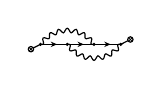
\begin{tikzpicture}[x=0.340cm, y=0.340cm, line width=0.420pt, baseline={([yshift=-0.6ex]0,0)}]
  \draw (-0.500,0.000) -- (0.500,0.000);
  \fill (0.119,0.000) -- (-0.119,0.102) -- (-0.042,0.000) -- (-0.119,-0.102) -- cycle;
  \draw (-1.500,0.000) -- (-0.500,0.000);
  \fill (-0.881,0.000) -- (-1.119,0.102) -- (-1.042,0.000) -- (-1.119,-0.102) -- cycle;
  \draw (0.500,0.000) -- (1.500,0.000);
  \fill (1.119,0.000) -- (0.881,0.102) -- (0.958,0.000) -- (0.881,-0.102) -- cycle;
  \draw plot[smooth, tension=0.7] coordinates {(0.500,0.000) (0.431,-0.003) (0.390,0.012) (0.385,0.055) (0.402,0.122) (0.417,0.190) (0.404,0.236) (0.358,0.247) (0.290,0.230) (0.224,0.210) (0.180,0.214) (0.164,0.254) (0.165,0.323) (0.161,0.393) (0.138,0.434) (0.090,0.433) (0.029,0.400) (-0.030,0.363) (-0.073,0.356) (-0.099,0.391) (-0.116,0.458) (-0.137,0.525) (-0.170,0.559) (-0.216,0.546) (-0.267,0.498) (-0.315,0.448) (-0.355,0.429) (-0.389,0.457) (-0.422,0.518) (-0.459,0.577) (-0.500,0.601) (-0.541,0.577) (-0.578,0.518) (-0.611,0.457) (-0.645,0.429) (-0.685,0.448) (-0.733,0.498) (-0.784,0.546) (-0.830,0.559) (-0.863,0.525) (-0.884,0.458) (-0.901,0.391) (-0.927,0.356) (-0.970,0.363) (-1.029,0.400) (-1.090,0.433) (-1.138,0.434) (-1.161,0.393) (-1.165,0.323) (-1.164,0.254) (-1.180,0.214) (-1.224,0.210) (-1.290,0.230) (-1.358,0.247) (-1.404,0.236) (-1.417,0.190) (-1.402,0.122) (-1.385,0.055) (-1.390,0.012) (-1.431,-0.003) (-1.500,0.000)};
  \draw plot[smooth, tension=0.7] coordinates {(-0.500,0.000) (-0.431,0.003) (-0.390,-0.012) (-0.385,-0.055) (-0.402,-0.122) (-0.417,-0.190) (-0.404,-0.236) (-0.358,-0.247) (-0.290,-0.230) (-0.224,-0.210) (-0.180,-0.214) (-0.164,-0.254) (-0.165,-0.323) (-0.161,-0.393) (-0.138,-0.434) (-0.090,-0.433) (-0.029,-0.400) (0.030,-0.363) (0.073,-0.356) (0.099,-0.391) (0.116,-0.458) (0.137,-0.525) (0.170,-0.559) (0.216,-0.546) (0.267,-0.498) (0.315,-0.448) (0.355,-0.429) (0.389,-0.457) (0.422,-0.518) (0.459,-0.577) (0.500,-0.601) (0.541,-0.577) (0.578,-0.518) (0.611,-0.457) (0.645,-0.429) (0.685,-0.448) (0.733,-0.498) (0.784,-0.546) (0.830,-0.559) (0.863,-0.525) (0.884,-0.458) (0.901,-0.391) (0.927,-0.356) (0.970,-0.363) (1.029,-0.400) (1.090,-0.433) (1.138,-0.434) (1.161,-0.393) (1.165,-0.323) (1.164,-0.254) (1.180,-0.214) (1.224,-0.210) (1.290,-0.230) (1.358,-0.247) (1.404,-0.236) (1.417,-0.190) (1.402,-0.122) (1.385,-0.055) (1.390,-0.012) (1.431,0.003) (1.500,0.000)};
  \draw (-1.500,0.000) -- (-1.857,-0.181);
  \draw[fill=white] (-1.857,-0.181) circle (0.100);
  \draw[line width=0.298pt] (-1.787,-0.111) -- (-1.927,-0.251) (-1.787,-0.251) -- (-1.927,-0.111);
  \draw (1.500,0.000) -- (1.857,0.181);
  \draw[fill=white] (1.857,0.181) circle (0.100);
  \draw[line width=0.298pt] (1.927,0.251) -- (1.787,0.111) (1.927,0.111) -- (1.787,0.251);
  \fill (0.500,0.000) circle (0.064);
  \fill (-0.500,0.000) circle (0.064);
  \fill (1.500,0.000) circle (0.064);
  \fill (-1.500,0.000) circle (0.064);
\end{tikzpicture}}
\diagramgap
\mbox{$\displaystyle -\,\frac{1}{4}$\,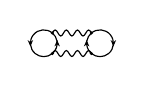
\begin{tikzpicture}[x=0.340cm, y=0.340cm, line width=0.420pt, baseline={([yshift=-0.6ex]0,0)}]
  \draw (-0.729,-0.383) arc[start angle=310.000, end angle=410.000, radius=0.500];
  \fill (-0.550,0.119) -- (-0.652,-0.119) -- (-0.550,-0.042) -- (-0.448,-0.119) -- cycle;
  \draw (-0.729,0.383) arc[start angle=50.000, end angle=310.000, radius=0.500];
  \fill (-1.550,-0.119) -- (-1.448,0.119) -- (-1.550,0.042) -- (-1.652,0.119) -- cycle;
  \draw (0.729,-0.383) arc[start angle=230.000, end angle=130.000, radius=0.500];
  \fill (0.550,0.119) -- (0.448,-0.119) -- (0.550,-0.042) -- (0.652,-0.119) -- cycle;
  \draw (0.729,0.383) arc[start angle=130.000, end angle=-130.000, radius=0.500];
  \fill (1.550,-0.119) -- (1.652,0.119) -- (1.550,0.042) -- (1.448,0.119) -- cycle;
  \draw plot[smooth, tension=0.7] coordinates {(-0.729,0.383) (-0.677,0.463) (-0.625,0.495) (-0.572,0.463) (-0.520,0.383) (-0.468,0.304) (-0.416,0.271) (-0.364,0.304) (-0.312,0.383) (-0.260,0.463) (-0.208,0.495) (-0.156,0.463) (-0.104,0.383) (-0.052,0.304) (0.000,0.271) (0.052,0.304) (0.104,0.383) (0.156,0.463) (0.208,0.495) (0.260,0.463) (0.312,0.383) (0.364,0.304) (0.416,0.271) (0.468,0.304) (0.520,0.383) (0.572,0.463) (0.625,0.495) (0.677,0.463) (0.729,0.383)};
  \draw plot[smooth, tension=0.7] coordinates {(-0.729,-0.383) (-0.677,-0.304) (-0.625,-0.271) (-0.572,-0.304) (-0.520,-0.383) (-0.468,-0.463) (-0.416,-0.495) (-0.364,-0.463) (-0.312,-0.383) (-0.260,-0.304) (-0.208,-0.271) (-0.156,-0.304) (-0.104,-0.383) (-0.052,-0.463) (0.000,-0.495) (0.052,-0.463) (0.104,-0.383) (0.156,-0.304) (0.208,-0.271) (0.260,-0.304) (0.312,-0.383) (0.364,-0.463) (0.416,-0.495) (0.468,-0.463) (0.520,-0.383) (0.572,-0.304) (0.625,-0.271) (0.677,-0.304) (0.729,-0.383)};
  \fill (-0.729,0.383) circle (0.064);
  \fill (-0.729,-0.383) circle (0.064);
  \fill (0.729,0.383) circle (0.064);
  \fill (0.729,-0.383) circle (0.064);
\end{tikzpicture}}
\diagramgap
\mbox{$\displaystyle +\,$\,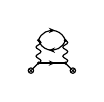
\begin{tikzpicture}[x=0.340cm, y=0.340cm, line width=0.420pt, baseline={([yshift=-0.6ex]0,0)}]
  \draw (-0.500,0.850) arc[start angle=162.811, end angle=17.189, radius=0.523];
  \fill (0.119,1.219) -- (-0.119,1.321) -- (-0.042,1.219) -- (-0.119,1.117) -- cycle;
  \draw (0.500,0.850) arc[start angle=342.811, end angle=197.189, radius=0.523];
  \fill (-0.119,0.481) -- (0.119,0.379) -- (0.042,0.481) -- (0.119,0.583) -- cycle;
  \draw (-0.500,0.000) -- (0.500,0.000);
  \fill (0.119,0.000) -- (-0.119,0.102) -- (-0.042,0.000) -- (-0.119,-0.102) -- cycle;
  \draw plot[smooth, tension=0.7] coordinates {(0.500,0.850) (0.565,0.808) (0.592,0.765) (0.565,0.722) (0.500,0.680) (0.435,0.638) (0.408,0.595) (0.435,0.552) (0.500,0.510) (0.565,0.467) (0.592,0.425) (0.565,0.382) (0.500,0.340) (0.435,0.298) (0.408,0.255) (0.435,0.213) (0.500,0.170) (0.565,0.127) (0.592,0.085) (0.565,0.042) (0.500,0.000)};
  \draw plot[smooth, tension=0.7] coordinates {(-0.500,0.850) (-0.435,0.808) (-0.408,0.765) (-0.435,0.722) (-0.500,0.680) (-0.565,0.638) (-0.592,0.595) (-0.565,0.552) (-0.500,0.510) (-0.435,0.467) (-0.408,0.425) (-0.435,0.382) (-0.500,0.340) (-0.565,0.298) (-0.592,0.255) (-0.565,0.213) (-0.500,0.170) (-0.435,0.127) (-0.408,0.085) (-0.435,0.042) (-0.500,0.000)};
  \draw (-0.500,0.000) -- (-0.783,-0.283);
  \draw[fill=white] (-0.783,-0.283) circle (0.100);
  \draw[line width=0.298pt] (-0.713,-0.213) -- (-0.853,-0.353) (-0.713,-0.353) -- (-0.853,-0.213);
  \draw (0.500,0.000) -- (0.783,-0.283);
  \draw[fill=white] (0.783,-0.283) circle (0.100);
  \draw[line width=0.298pt] (0.853,-0.213) -- (0.713,-0.353) (0.853,-0.353) -- (0.713,-0.213);
  \fill (0.500,0.850) circle (0.064);
  \fill (-0.500,0.850) circle (0.064);
  \fill (0.500,0.000) circle (0.064);
  \fill (-0.500,0.000) circle (0.064);
\end{tikzpicture}}
